% !TeX spellcheck = cs_CZ
{\tikzset{external/prefix={tikz/FYZI/}}
 \tikzset{external/figure name/.add={ch24_}{}}
%=========================== Kapitola: Přechodové jevy ============================================
\chapter{Přechodové jevy}\label{fyz:IchapXXIV}
\minitoc
  \section{Energie oscilátoru}\label{fyz:IchapXXIVsecI}
  \section{Tlumené kmity}\label{fyz:IchapXXIVsecII}
  \section{Přechodové jevy v elektrických obvodech}\label{fyz:IchapXXVIVsecIII}
  \section{Příklady a cvičení}\label{fyz:IchapXXIVsecIV}

    \begin{figure}[ht!] %\ref{fyz:fig300}
      \centering
      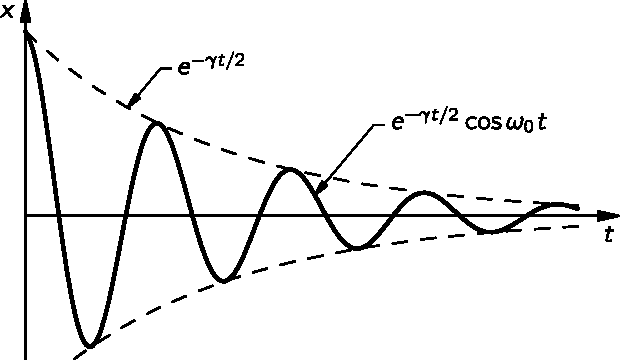
\includegraphics[width=0.7\linewidth]{fyz_fig300.pdf}
      \caption{Tlumené kosinové oscilace 
               (\cite[s.~326]{Feynman01})}
      \label{fyz:fig300}
    \end{figure}

    \begin{figure}[ht!] %\ref{fyz:fig301}
      \centering
      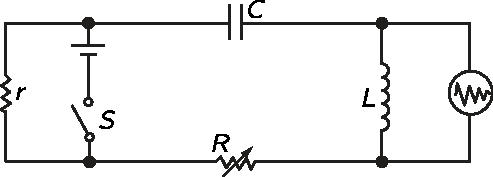
\includegraphics[width=0.7\linewidth]{fyz_fig301.pdf}
      \caption{Demonstrace přechodových jevů na elektrickém obvodu 
               (\cite[s.~328]{Feynman01})}
      \label{fyz:fig301}
    \end{figure}
    

    \begin{figure}[ht!]      %\ref{fyz:fig302}
      \centering
      \begin{tabular}{cc}
        \subfloat[ ]{\label{fyz:fig302a}
          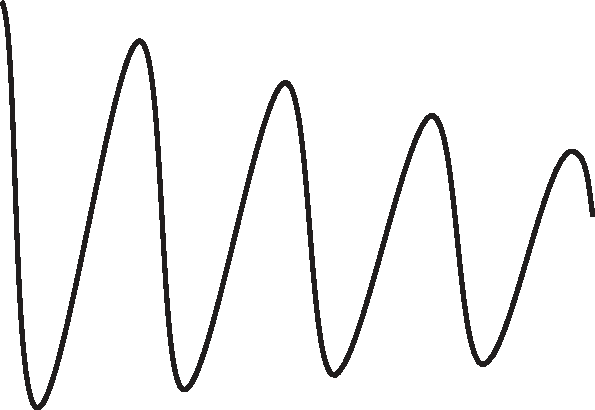
\includegraphics[width=0.4\linewidth]{fyz_fig302a.pdf}}
        \hspace{-1em}                                                       &
        \subfloat[ ]{\label{fyz:fig302b}
          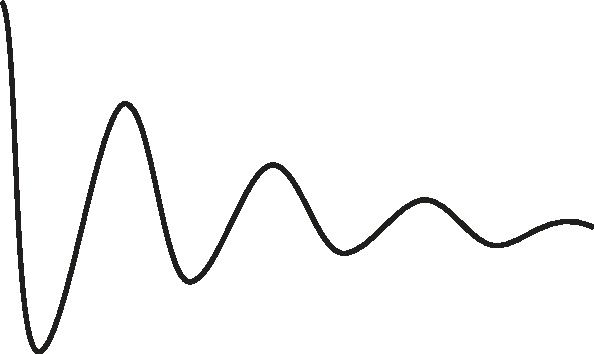
\includegraphics[width=0.4\linewidth]{fyz_fig302b.pdf}}         \\
        \subfloat[ ]{\label{fyz:fig302c}
          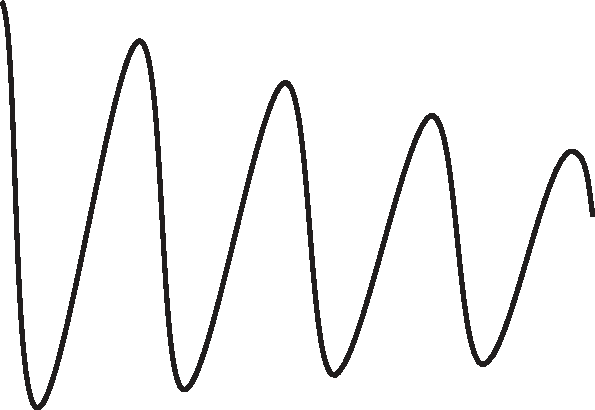
\includegraphics[width=0.4\linewidth]{fyz_fig302a.pdf}}
        \hspace{-1em}                                                       &
        \subfloat[ ]{\label{fyz:fig302d}
          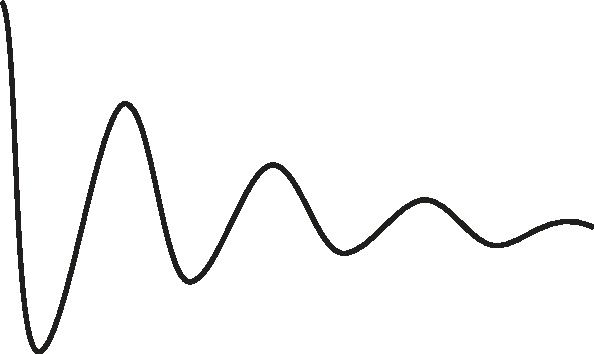
\includegraphics[width=0.4\linewidth]{fyz_fig302b.pdf}}         
      \end{tabular}
      \caption{Příklady tlumených oscilací vyfotografovaných z obrazovky osciloskopu
               \cite[s.~329]{Feynman01}}
      \label{fyz:fig302}
    \end{figure}

} %tikzset
%---------------------------------------------------------------------------------------------------
\printbibliography[title={Seznam literatury}, heading=subbibliography]
\addcontentsline{toc}{section}{Seznam literatury}